\documentclass[a4paper,conference]{IEEEtran}
\IEEEoverridecommandlockouts
\usepackage{cite}
%\usepackage{sectsty}
\usepackage{amsmath,amssymb,amsfonts}
\usepackage{algorithmic}
\newcommand{\todo}[1]{\color{red}TODO:\textbf{#1}\color{black}}
\usepackage{graphicx}
\usepackage{textcomp}
\usepackage{xcolor}
\usepackage{hyperref}
\usepackage{tabularx}
\usepackage{IEEEtrantools}
\usepackage{lettrine}
\usepackage{caption}
\usepackage{fancyhdr}
\def\BibTeX{{\rm B\kern-.05em{\sc i\kern-.025em b}\kern-.08em
    T\kern-.1667em\lower.7ex\hbox{E}\kern-.125emX}}

\usepackage{scalerel}
\usepackage{tikz}

\usetikzlibrary{svg.path}

\definecolor{orcidlogocol}{HTML}{A6CE39}
\tikzset{
  orcidlogo/.pic={
    \fill[orcidlogocol] svg{M256,128c0,70.7-57.3,128-128,128C57.3,256,0,198.7,0,128C0,57.3,57.3,0,128,0C198.7,0,256,57.3,256,128z};
    \fill[white] svg{M86.3,186.2H70.9V79.1h15.4v48.4V186.2z}
                 svg{M108.9,79.1h41.6c39.6,0,57,28.3,57,53.6c0,27.5-21.5,53.6-56.8,53.6h-41.8V79.1z M124.3,172.4h24.5c34.9,0,42.9-26.5,42.9-39.7c0-21.5-13.7-39.7-43.7-39.7h-23.7V172.4z}
                 svg{M88.7,56.8c0,5.5-4.5,10.1-10.1,10.1c-5.6,0-10.1-4.6-10.1-10.1c0-5.6,4.5-10.1,10.1-10.1C84.2,46.7,88.7,51.3,88.7,56.8z};
  }
}

\newcommand\orcidicon[1]{\href{https://orcid.org/#1}{\mbox{\scalerel*{

\begin{tikzpicture}[yscale=-1,transform shape]
\pic{orcidlogo};
\end{tikzpicture}
}{|}}}}
\thispagestyle{fancy}
\pagestyle{fancy}
\fancyhf{}

\fancyfoot[L]{\ifnum\value{page}=1 979-8-3503-1324-6/23/\$31.000~\copyright2023 IEEE \fi} % Copyright notice only on the first page
\renewcommand{\headrulewidth}{0pt} % Remove the horizontal line in the header

   
\begin{document}

\thispagestyle{fancy}
\title{MINDTwin AI: Multiphysics Informed Digital-Twin for Fault Localization in Induction Motor using AI}
\thispagestyle{fancy}
\IEEEpubidadjcol

\makeatletter
\newcommand{\linebreakand}{%
  \end{@IEEEauthorhalign}
  \hfill\mbox{}\par
  \mbox{}\hfill\begin{@IEEEauthorhalign}
}
\makeatother
\author{ 
  \IEEEauthorblockN{Amina Bashir\IEEEauthorrefmark{1}, Muhammad Ahmed Mohsin\IEEEauthorrefmark{1} \orcidicon{0009-0005-2766-0345}\  }
  \IEEEauthorblockA{\textit{School of Electrical Engineering and Computer Science (SEECS),} \\
    \textit{National University of Sciences and Technology (NUST),}\\
    Islamabad, Pakistan \\
    \{abashir,mmohsin\}.bee20seecs@seecs.edu.pk
  }
  \and
  \IEEEauthorblockN{Muhammad Jazib\IEEEauthorrefmark{1}}
  \IEEEauthorblockA{\textit{Department of Electrical Engineering (DEE),} \\
    \textit{Pakistan Institute of Engineering and Applied Sciences,}\\
    Islamabad, Pakistan \\
    bsee2023@pieas.edu.pk
  }
  \linebreakand
  \IEEEauthorblockN{Hafsa Iqbal}
  \IEEEauthorblockA{\textit{School of Electrical Engineering and Computer Science (SEECS),} \\
    \textit{National University of Sciences and Technology (NUST),}\\
    Islamabad, Pakistan \\
    hafsa.iqbal@seecs.edu.pk
  }
}




\maketitle
\IEEEpubidadjcol
\thispagestyle{fancy}

\begin{abstract}
This paper focuses on an Artificial Intelligence (AI)-based approach for fault localization in a squirrel cage three-phase induction motor (TIM). A multifaceted Digital-Twin (DT) is designed by integrating physics domain knowledge with AI algorithms. The aim is to design a Multiphysics-informed hybrid DT for fault detection and localization in TIM. To achieve this, a high-fidelity computational model of an induction motor is developed using the Finite Element Analysis (FEA) in COMSOL Multiphysics. The model parameters, loading conditions, and boundary conditions are meticulously tuned with an experimental workbench using a Sparse Nonlinear Optimization (SNOPT) solver. Simulations are conducted to replicate various electrical and mechanical defects. Additionally, the model order reduction technique is employed to generate a reduced state-space model, enabling the high-fidelity dynamic system to act as a virtual sensor exhibiting real-time capabilities. The feature fusion process leverages Canonical Correlation Analysis (CCA) within the hybrid DT modeling framework. Comparative analysis demonstrates that the Multiphysics-informed hybrid modeling approach enhances the interpretability of AI classifiers, improving real-time condition monitoring and fault localization in TIM.
\end{abstract}
\let\thefootnote\relax\footnotetext{$^\ast$ The authors contributed equally and are co-first authors. The names are arranged alphabetically.}


\begin{IEEEkeywords}
Multiphysics, hybrid digital twin, finite element model, fault detection, Machine Learning, and Deep neural network.
\end{IEEEkeywords}

\section{Introduction}
\begin{figure*}[t!]
    \centering
    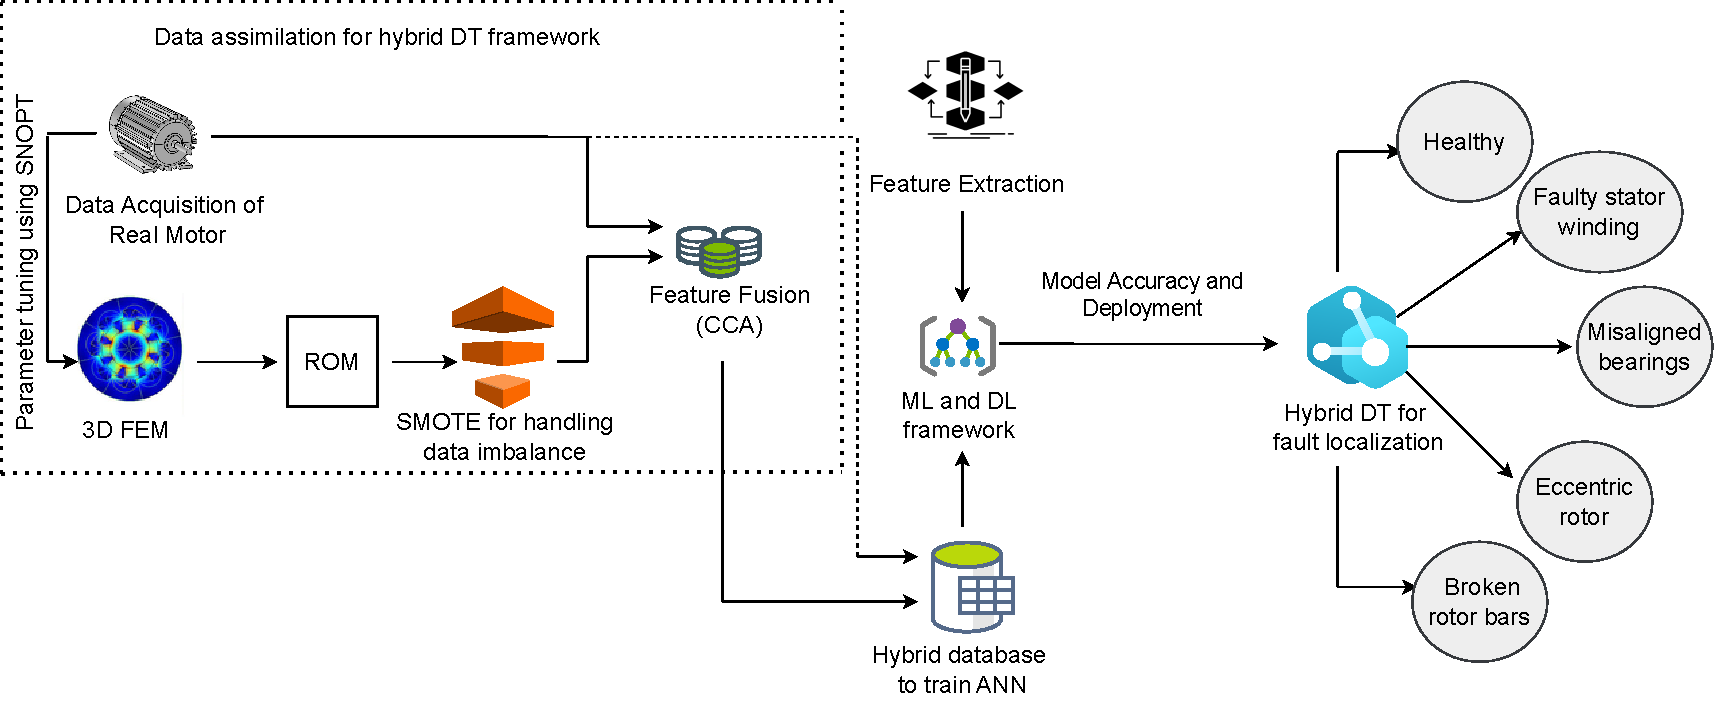
\includegraphics[width=0.8\textwidth]{Figs/hh.drawio.pdf}
    \caption{Workflow for integrating database of experimental TIM and Multiphysics FEM to develop Hybrid DT for fault localization.}
    \label{fig:DAQ}
\end{figure*}
\lettrine{I}{ndustry} 4.0 has ushered in an era where Digital-Twins (DT) represent one of the most prominent and transformative technologies. The DT holds the potential to revolutionize complex control systems by offering real-time condition monitoring, predictive maintenance, and fault prognosis capabilities. The need for DT becomes evident in the field of large-scale machines and complex dynamical systems to prevent invasive monitoring methods, energy losses, and unscheduled downtime~\cite{8930293}. Among the diverse array of electrical drives employed in industrial ecosystem, the three-phase squirrel cage induction motor (TIM) stands out as a significant contributor, accounting for $65\%$ of global energy consumption~\cite{GHOSH20201139}. These TIMs, however, are susceptible to various electrical and mechanical faults arising from malfunctions such as bearing abnormalities, mass imbalances, and circuit failure. To address evolving demands of the industrial landscape, a robust digitalized platform is required that encompasses integration, computing capabilities, data infrastructure, repositories, and advanced analytics for efficient and sophisticated condition monitoring in TIMs. Traditionally, DTs have been trained solely with datasets obtained from of real-world dynamic systems. However, big data alone is not enough, as DT must incorporate domain knowledge of physics to effectively model these complex systems. This leads to the concept of physics-enhanced machine learning~\cite{pawar2021hybrid} to develop a hybrid DT that combines both data-driven and physics-driven models. In this paper, we propose an efficient hybrid DT that incorporates the following approaches:


\textbf{Physics-driven modeling:} A physics-driven model is designed on well-defined principles of mathematics and classical physics. This approach addresses real-time data sparsity and data uncertainty encountered in complex dynamical systems. In our work, we have employed the COMSOL Multiphysics software to design a high-fidelity Finite Element Model (FEM). This framework incorporates fundamental principles such as electromagnetic field theory and multibody dynamics. The physical interfaces within the model are coupled using differential equations and appropriate boundary conditions, resulting in a robust physics-driven model.


\textbf{Data-driven modeling:} Various sensors are installed on different components of both healthy and faulty motors to measure key variables, including vibrations at the motor's drive and non-drive ends, as well as stator currents and voltages. The data collected from sensors are processed and fed into AI models. These AI models are trained to map input data from TIM to corresponding fault labels.


\textbf{Reduced order modeling (ROM):} The high-fidelity FEM is defined using a large set of mathematical equations and complex geometry, which results in slowing down the simulation. To enable the DT to function as a virtual sensor with real-time capabilities, a projection-based ROM~\cite{9982890} is employed. This reduces the model's dimensionality and order, ensuring efficient real-time performance. 

Our work proposes a hybrid DT that leverages data-driven and physics-driven approaches for fault localization in a squirrel cage TIM. A high-level overview of the proposed design is shown in Fig.~\ref{fig:DAQ}. The proposed design undergoes design optimization and parameter tuning to calibrate FEM to the actual motor. To address real-time data sparsity, synthetic data generated by the FEM is incorporated. Fusing experimental and synthetic datasets results in a comprehensive database, serving as the foundation for training our hybrid DT.



\section{Literature review}
In the context of Industry 4.0, hybrid DT aims to create a virtual copy of a physical system for real-time condition monitoring, predictive maintenance, and diagnosis of faults and abnormalities. Within the domain of TIM, several approaches have been proposed to integrate the FEM for fault detection. \textit{Physics-informed neural networks} are proposed to improve the interpretability of ML models~\cite{9646258}. This approach capitalizes on the synergy between physics-driven and data-driven techniques, aligning with the broader objective of hybrid DTs.
\iffalse 
A framework for hybrid DT that integrates both data-driven and physics-driven approaches is proposed, so the hybrid DT leverages the best available technologies from physics simulation and data modeling.
\fi 
\textit{FEM-based approaches} generate a synthetic database to distinguish the fault severity in TIMs~\cite{8930293}. The research compares the FEM-based fault detection approach, FEM coupled with signal processing-based approach, and FEM with AI-based approach.  Another approach uses the \textit{two-dimensional (2D) FEA} to model broken rotor bars (BRB)~\cite{8369981}. This approach leverages finite element simulations to investigate malfunctioning severities. ML methods are subsequently employed to classify these malfunctions, highlighting the valuable insights that ML can offer for fault prognosis. 

The energy efficiency Digital Shadow of the induction motor is analyzed using the \textit{Adaptive Neuro-Fuzzy Inference System (ANFIS) algorithm}~\cite{AMADOUADAMOU2023101469}. This approach incorporates a simulated TIM equivalent circuit, resulting in a hybrid approach. The root-mean-square error between the estimated and measured results is $0.205$, highlighting the potential of hybrid models in addressing energy efficiency. Moreover, \textit{Three-dimensional (3D) FEM simulations} are also integrated with multi-layer perceptron (MLP) neural network architecture~\cite{s21237833} for BRB classification using Motor Current Signature Analysis (MCSA) in time and frequency domains. These results underscore the utility of digital data obtained from FEM simulations in the efficient design of DT. 

\textbf{Contributions:} In this paper, we propose a novel approach to develop a hybrid DT for classifying various faults in TIM. The primary contributions of this work are as follows:
\begin{itemize}
    \item Most of the mentioned research work employs 2D FEM of the motor. In contrast, our research uses a 3D Multiphysics FEM to couple the multibody dynamics and model rotating components of TIM. The database consists of four fault classes, enabling the hybrid DT to detect a wide range of electrical and mechanical faults. 
    \item We implement ROM and integrate it with other techniques, such as design optimization and spectral feature extraction, to improve the computational efficiency of the model. Canonical Correlation Analysis is utilized to fuse features from experimental and simulated workbenches. 
    \item We provide a novel comparative analysis between traditional data-driven and proposed hybrid models, highlighting the hybrid DT's efficiency.
\end{itemize}
\begin{figure*}[h!]
    \centering
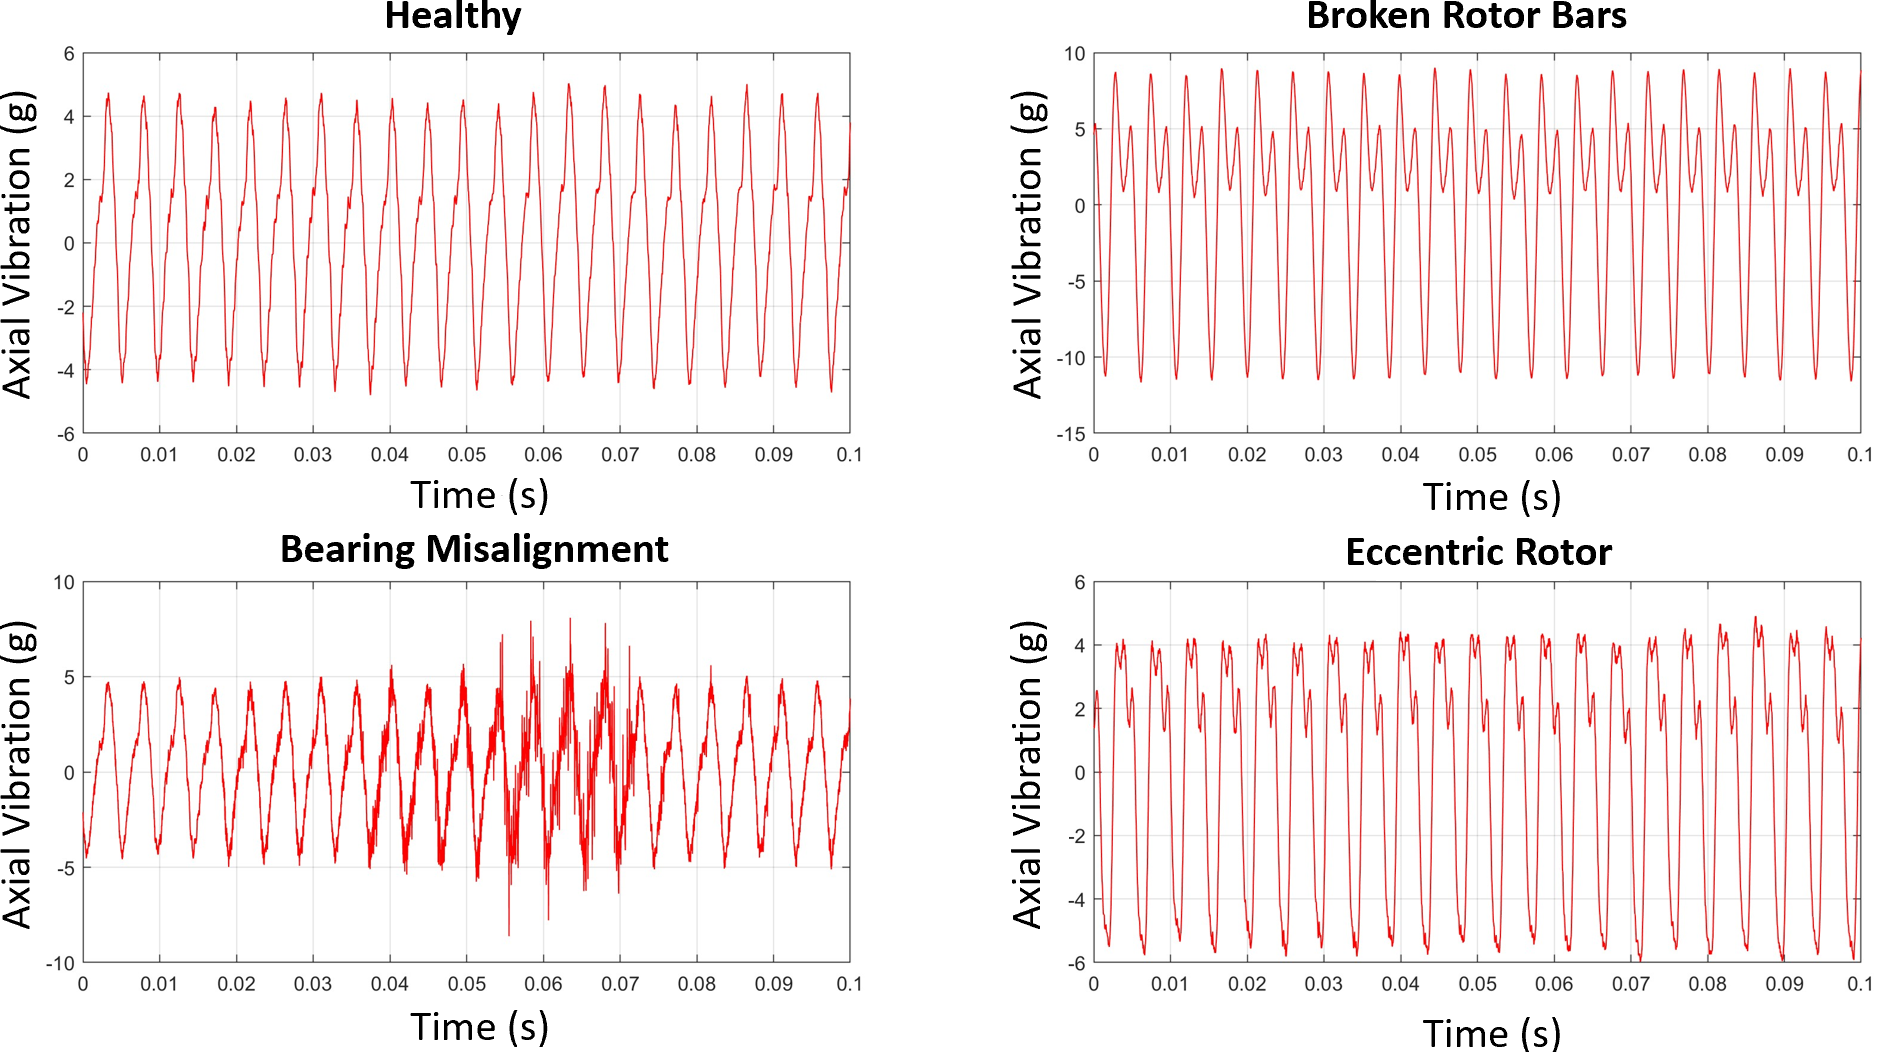
\includegraphics[width=0.8\textwidth]{Figs/attempt22.png}
\caption{Experimental datasets: time domain axial vibrations corresponding to healthy and faulty motors with broken rotor bars, bearing misalignment and eccentric rotors shown in sub-figures, respectively.}
    \label{fig:flowchart}
\end{figure*}

\begin{table}[b!]
    \centering
    \setlength{\arrayrulewidth}{0.3pt} % Adjust the table border thickness
    \caption{PARAMETERS OF EXPERIMENTAL WORKBENCH OF TIM.}
    \resizebox{0.70\columnwidth}{!}{\begin{tabular}{ll}
            \hline
            \textbf{Motor Parameters} & \textbf{Value} \\
            \hline
            Power Rating        & 1 hp   \\
            Voltage             & 220 V  \\
            Current             & 3.02 A \\
            Number of Poles     & 4     \\
            Frequency           & 60 Hz  \\
            Steady State Torque & 4.1 Nm \\
            Rated Speed         & 1715 RPM \\
            Rotor Slip          & 4.72 \%\\ 
            \hline
        \end{tabular}}
    \label{tab:motor-specifications}
\end{table}

\textbf{Paper Organization:} Section~\ref{sec:databaseGeneration} discusses the database generation of healthy and faulty TIMs using experimental setup and FEM simulations. Section~\ref{sec:virtualFEM} indicates how FEM is calibrated to real-life motor using design optimization and model order reduction.
Section~\ref{sec:dataAssimilation} describe the data assimilation methods employs to design hybrid database for fault localization (section~\ref{sec:FaulLocalization}) and offset prediction (section~\ref{sec:OffsetPrediciton}). Quantitative comparison is provided in section~\ref{sec:quantitativeAnalysis} which indicates that the proposed hybrid DT model outperforms the traditional DT models. Finally, section~\ref{sec:conclusion} concludes this work and provides insights for future tasks. 


\section{Database Generation for Hybrid DT} \label{sec:databaseGeneration}
Three-phase stator currents and voltages, axial and radial vibrations, and torque data were recorded to create the dataset. It includes real-time data from three types of motors: healthy, two with broken rotor bars~\cite{Huang2018-rk}, misaligned bearings~\cite{fmnm-bn95-20}, and eccentric rotors. The coil-ground faults in stator windings were modeled in COMSOL Multiphysics software, due to the unavailability of real-time data for faulty windings was unavailable. Moreover, FEM datasets were used to supplement the sparse variables like torque, stator currents, and voltages in motors with misaligned bearings and eccentric rotors. The following subsections discuss the experimental setup and FEM approaches employed to generate real-time and simulated datasets for healthy and faulty TIM.



\subsection{Data Acquisition for Experimental Workbench}
The experimental workbench consists of a squirrel cage TIM coupled to a DC generator with full bridge rectification in its winding. This setup enables a parametric sweep from steady to transient under a load torque varied from $0.5$ Nm to $4.1$ Nm. Frequency converters are used to monitor the motor's response to varying frequencies. Detailed motor parameters are shown in Table~\ref{tab:motor-specifications}.

\begin{figure}[b!]
    \centering
    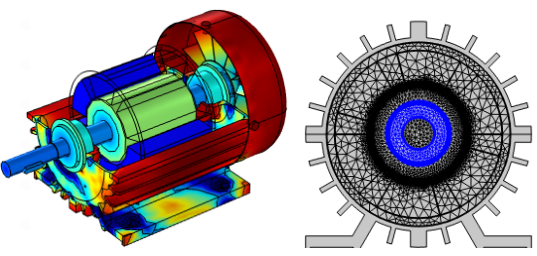
\includegraphics[width=0.45\textwidth]{Figs/combine_images.png}
    \caption{A 3D model of squirrel cage TIM is simulated using FEA and the corresponding 2D front view illustrating the mesh configuration in COMSOL Multiphysics.}
    \label{fig:FEM}
\end{figure}

Clamp-on probes are employed to measure electrical signals, while five axial accelerometers are used for vibrational analysis. Real-time data is collected for simulating three fault classes, two broken rotor bars~\cite{Huang2018-rk}, rotor eccentricity, and misaligned bearings~\cite{fmnm-bn95-20}. Sholes are drilled in two bars to observe the effects of broken rotor bars on the motor. For condition monitoring, $153,700$ data samples are collected for healthy and faulty motors, enabling vibrational analysis in axial and radial directions, and $200,000$ data samples for electrical analysis.  Datasets for inner race and outer defects are generated through repeated trials at a sampling frequency of $0.2$MHz, recording vibration and rotor angular speed. Fig.~\ref{fig:flowchart} shows a vibrational analysis of different faults in the physical motor setup. As evident from the plot, the healthy motor exhibits minimal axial vibrations. 
The motor's axial vibration with two broken rotor bars shows increased perturbation due to an asymmetric magnetic field. Bearing misalignment amplifies vibration by inducing stress and unbalanced loading conditions on the motor's shaft. The eccentricity of the rotor slipping causes an unbalanced distribution of mass along the rotor's circumference. The fault severity is prevalent as asymmetric centrifugal forces and reaction forces in the coupling induce vibrations along the rotor axis, as depicted in Fig.~\ref{fig:flowchart}. These vibrations lead to motor wear and tear and reduced efficiency.
\begin{figure}[t!]
    \centering    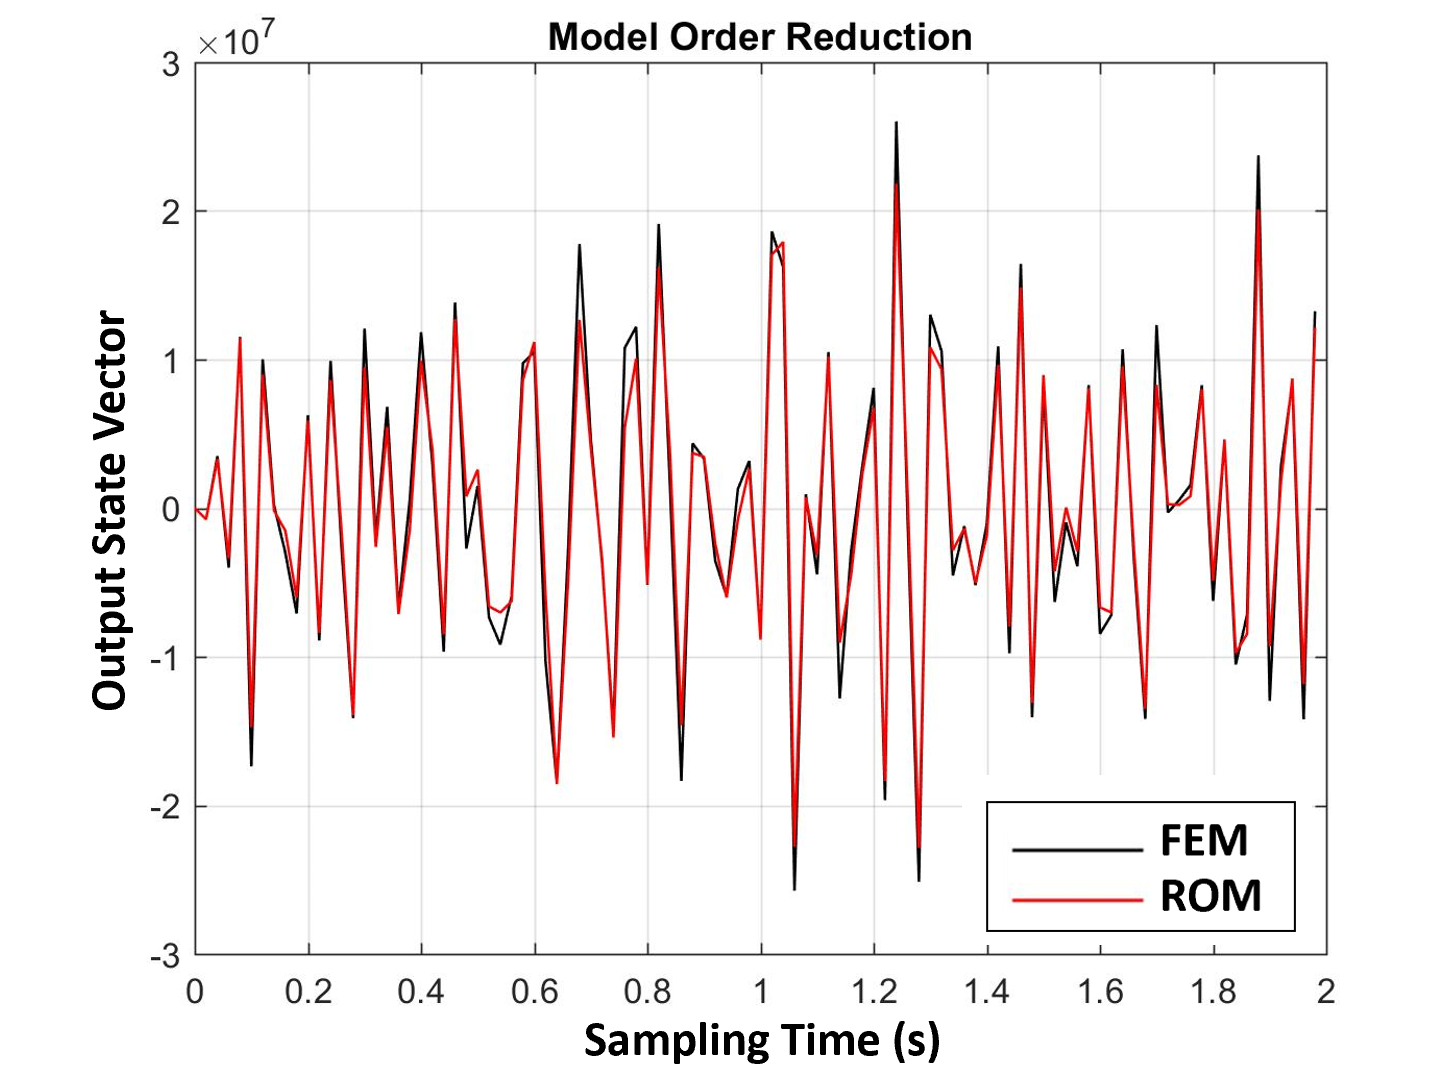
\includegraphics[width=0.45\textwidth]{ Figs/update2.png }
    \caption{ Comparison of Output State Vector between full order and reduced order FEM.}
    \label{fig:eccentrric}
\end{figure}


\subsection{FEM under Normal Operating Conditions}
A high-fidelity model for TIM~\cite{kocman2016induction} by coupling electrical circuits, rotating machinery, electromagnetic field theory, and multi-body dynamics is designed in COMSOL Multiphysics, as shown in Fig.~\ref{fig:FEM}. The mesh design is a combination of physics-controlled and user-controlled. The electromagnetic field equation computes the machine's dynamic behavior as follows;
\begin{equation}
\sigma \frac{\partial A}{\partial t} + \nabla \times H - \sigma (\mathbf{v} \times \mathbf{B}) = \mathbf{J}_e,
\end{equation}
where external current density $J_e$ is computed using partial derivative of magnetic vector potential $A$ with respect to time $t$, electric conductivity $\sigma$, rotor velocity $\mathbf{v}$, magnetic flux density $\mathbf{B}$, and curl $\nabla$ of magnetic flux intensity $\mathbf{H}$.
 \\
Maxwell’s stress tensor \(\tau\)~\cite{kocman2016induction}
 over the exterior surfaces of domains is used to calculate inner torque as follows:
\begin{equation}
\tau = \oint_{\partial\Omega} d(r - r_0) \times (\mathbf{n} \cdot \mathbf{T}) \, dS,
\end{equation}
where \(\mathbf{r} - \mathbf{r}_0\) is the displacement vector, \(\mathbf{n}\) is the normal vector and \(\mathbf{T}\) is the stress vector.


The rotor dynamics for the start-up~\cite{8778128} are modeled by:


\begin{equation}
\frac{d\omega_r}{dt} = \frac{T_r - T_L}{I}.
\end{equation}
\textbf{Misaligned bearing fault (outer and inner races): }

The equation expresses variation in angular speed $\omega_r$ during the motor start-up for a certain load torque $T_L$, where $I$ is inertia, and $T_r$ is inner electromagnetic torque. The parameters are adjusted for rotor speed to be $1715$ revolutions per minute (RPM) at full load.
\begin{figure}[t!]
    \centering
    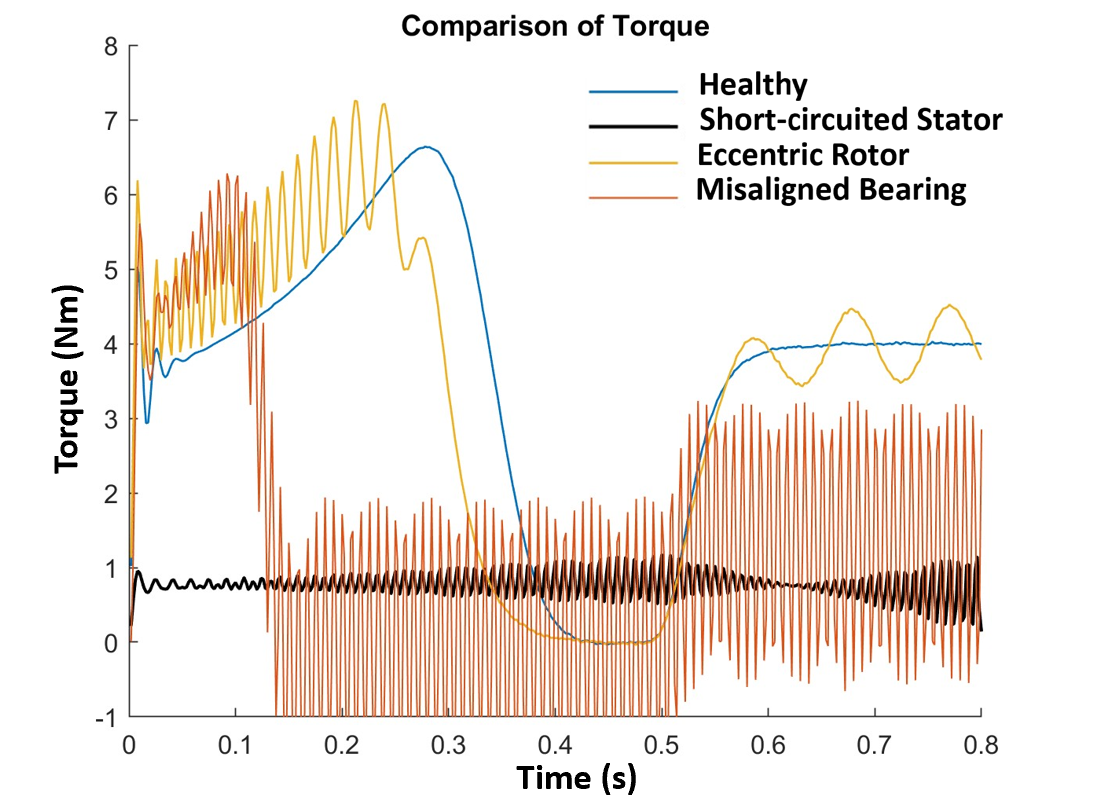
\includegraphics[width=0.45\textwidth]{Figs/UPDATE1.png }
    \caption{ A time-dependent analysis of torque under a rated load of $4.1$ Nm is simulated using FEA for both healthy and faulty motors with short-circuited stator, eccentric rotor, and misaligned bearings.}
    \label{fig:ROM}
\end{figure}

\begin{figure*}[t!]
    \centering
    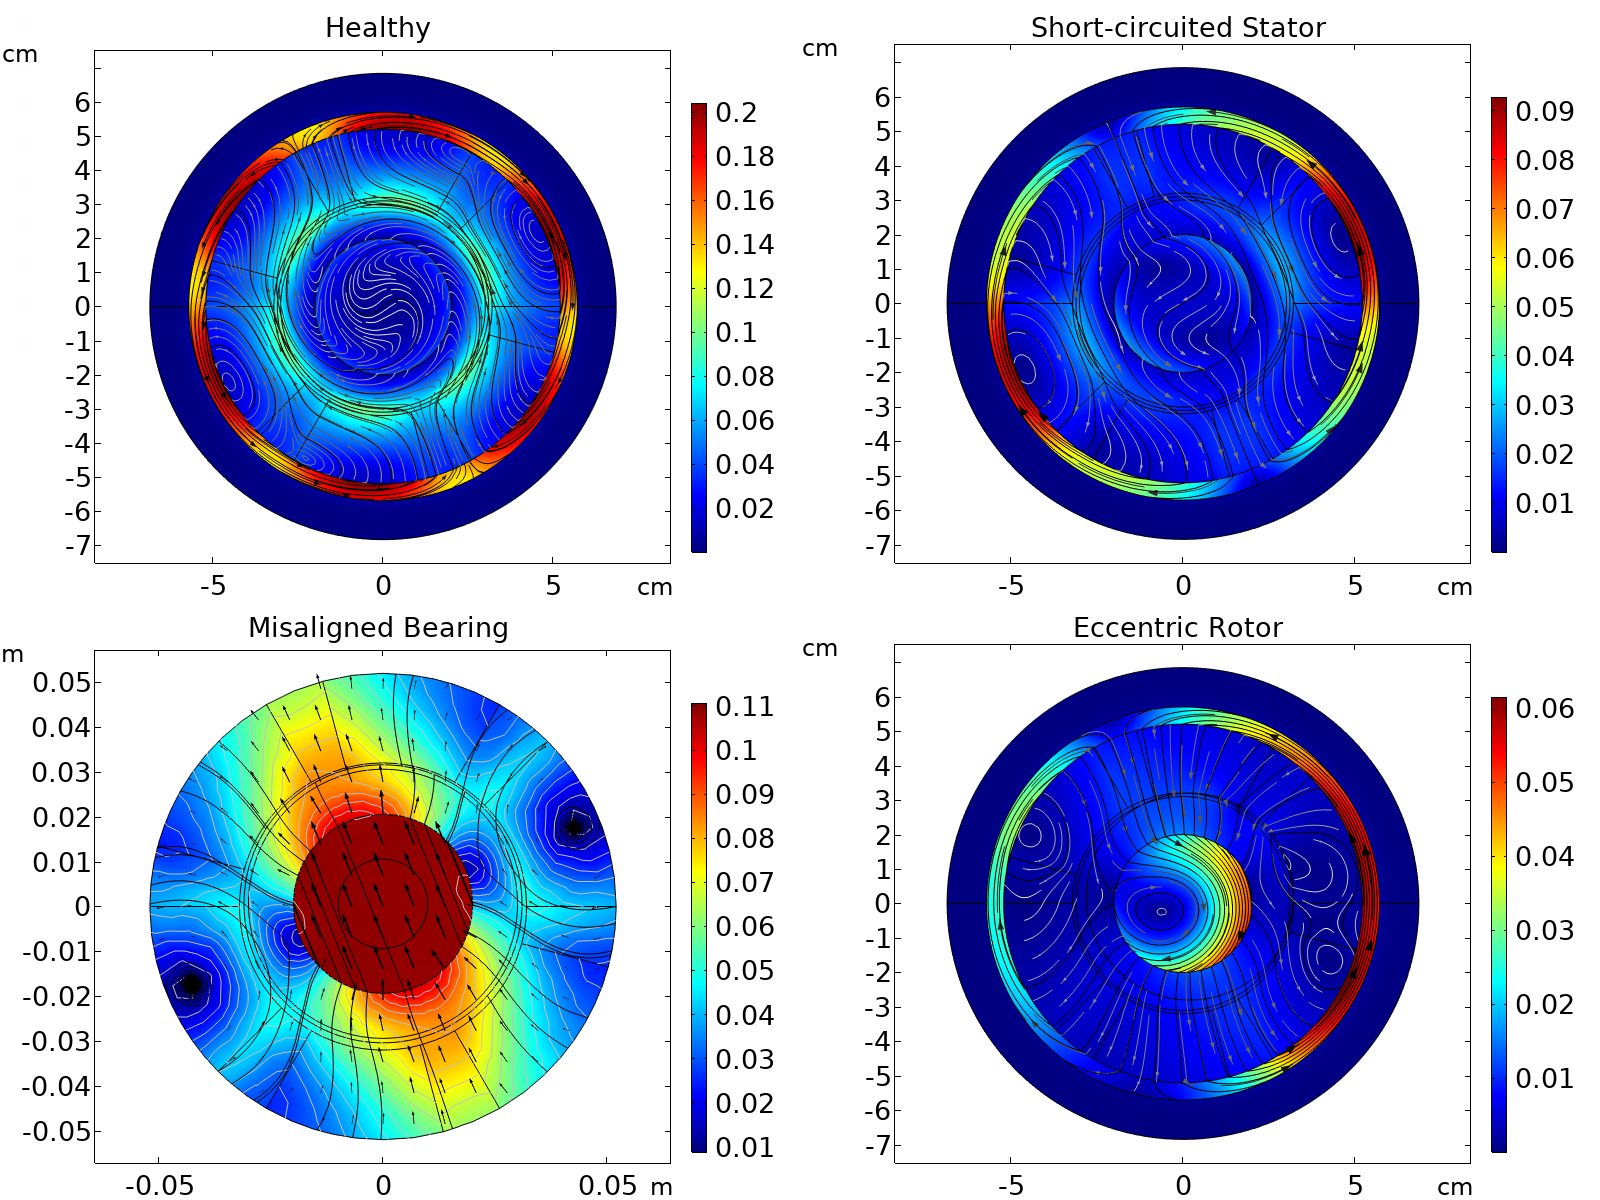
\includegraphics[width=0.8\textwidth]{ Figs/sp.png } 
    \caption{Comparison of magnetic flux density norm for healthy and faulty motors with short-circuited stator, misaligned bearing, and eccentric rotor. Arrows represent the flow of the magnetic field.}\label{fig:Torque}
\end{figure*}



\subsection{FEM under Fault Operating Conditions}
The parameters missing in real-time data sets are modeled using COMSOL to obtain a comprehensive database. The following three faulty motors are simulated in COMSOL;

\textbf{Stator winding fault (coil to ground):} The coil-ground fault is introduced in one phase of the TIM using an electrical circuit interface~\cite{8778128}. Stator faults lead to a deterioration in flux linkage $\Phi_s$ due to reductions in both stator current $i_s$ and rotor current $i_R$, as described by the following equation:
\begin{equation}
\Phi_s = L_s \cdot i_s + L_m \cdot i_{R} \cdot e^{j\omega t},
\end{equation}
where $\omega$ is angular frequency of sinusoidal signal, $L_s$ is stator inductance and $L_m$ is mutual inductance between stator and rotor winding.
Stator faults induce abnormal vibrations in motor torque, leading to unbalanced time-harmonic currents flowing through the other phases of stator windings. Since torque is directly proportional to magnetic field strength, the torque, and magnetic field intensity are reduced for stator winding faults due to flux leakages. Additionally, the current imbalance results in a surge in one phase of the stator and affects the other phase currents.



An offset value is used to displace two bearings to cause mass imbalance. Moreover, the damping coefficients of bearings are also reduced to model the abnormality. 
Passage frequency for inner race $f_{\text{PE}}$ and outer race $f_{\text{PI}}$ depends on bearing elements $N_b$, diameter ratio of elements $D_b/D_c$, the angle between bearing elements $\beta$, and $f_R$ is the rotational frequency~\cite{wu2020automatic}:
\begin{equation}
f_{\text{PE}},f_{\text{PI}}  = \frac{N_b}{2}f_{\text{R}}\left(1 \pm \frac{D_{\text{b}}}{D_{\text{c}}}\cos(\beta)\right).
\end{equation}

The misaligned bearings cause inner race and outer race defects in TIM. The motor transient to steady state response for misaligned bearing shows angular speed and torque perturbations. 



\textbf{Eccentric rotor fault (non-uniform air gap density):} The mechanical deterioration is modeled by displacing the axial center of the rotor from (0,0) to (1,1), which results in a non-uniform air gap~\cite{tian2018induction}. The magnetic field is sparse for wide air gaps. The torques of faulty models show oscillations at a full load condition of $4.1$Nm during the motor’s transient to steady state response. %The arrow lines show field flow disruption due to a non-uniform air gap created by misalignment \todo{arrow lines in fig.6? if yes, then please refer the figure here}.

\textbf{Analysis of torque and magnetic field density for FEM simulations:} Normal motor exhibits a uniform and symmetric magnetic field, as depicted in Fig.~\ref{fig:ROM} and Fig.~\ref{fig:Torque}.  The start-up torque of a healthy motor reaches a steady state after 0.5 seconds. In TIM with the short-circuited stator, the electromagnetic coupling reduces since a secondary path is available for the stator current to flow, reducing the torque. An imbalance in a magnetic field can be seen in Fig.~\ref{fig:Torque} in one coil phase, subject to torque reduction and increased stator winding losses. The misaligned bearings cause fluctuations in torque because uneven forces act on the bearing. Bearing misalignment has altered the uniformity of the magnetic field. An uneven mass distribution in the eccentric rotor causes an unbalanced response, resulting in perturbation in axial forces, which causes the rotor to wobble. This explains the fluctuations in torque. The magnetic field loses its uniformity in stator since opposing eddy currents induced in the core cause additional losses. The arrow lines in Fig.~\ref{fig:Torque} show rotor misalignment creates a field flow disruption due to a non-uniform air gap.






\section{Reduced Order FEM as Real-time Virtual Sensor}\label{sec:virtualFEM}

A high-fidelity dynamic system requires greater computational time because of a higher degree of freedom (DOF). FEMs that we have designed require high computational resources and greater execution time. This section presents how FEM can serve as a virtual sensor with real-time efficiency. 
To achieve real-time capabilities, state-of-the-art reduction algorithms using sparse state-space Model Order Reduction (sssMOR) toolbox~\cite{castagnotto2017sss} are employed to capture features of our TIM's complex dynamic system without compromising the model's accuracy. The state-space extraction for TIM is given by:
\begin{align}
M_{c}(\dot{x}) &= M_{c} \cdot A\cdot{x} + M_{c} \cdot B\cdot{u}, \label{eq:equation1} \\
y &= C\cdot{x} + D\cdot{u}, \label{eq:equation2}
\end{align}
where output variables $y$ comprise current density, magnetic flux density, electromagnetic forces on the rotor, and torque. The input variables $u$ are power source frequency, current amplitude, and load torque. $M_c$ is the elimination matrix for the finite-element assembly for essentially relevant constraints and DOF. The state-space model extraction is followed by model order reduction using sparse state-space model order reduction (sssMOR) toolbox~\cite{castagnottosss} through co-simulation of COMSOL model in MATLAB. The error is calculated to 0.4464\%. Fig.~\ref{fig:eccentrric} depicts that output state vectors corresponding to the actual FEM and ROM match substantially. Table~\ref{tab:dof} shows that a precise prediction capability for ROM is achieved with only 2000 DOF.



 \begin{figure}[b!]
    \centering
    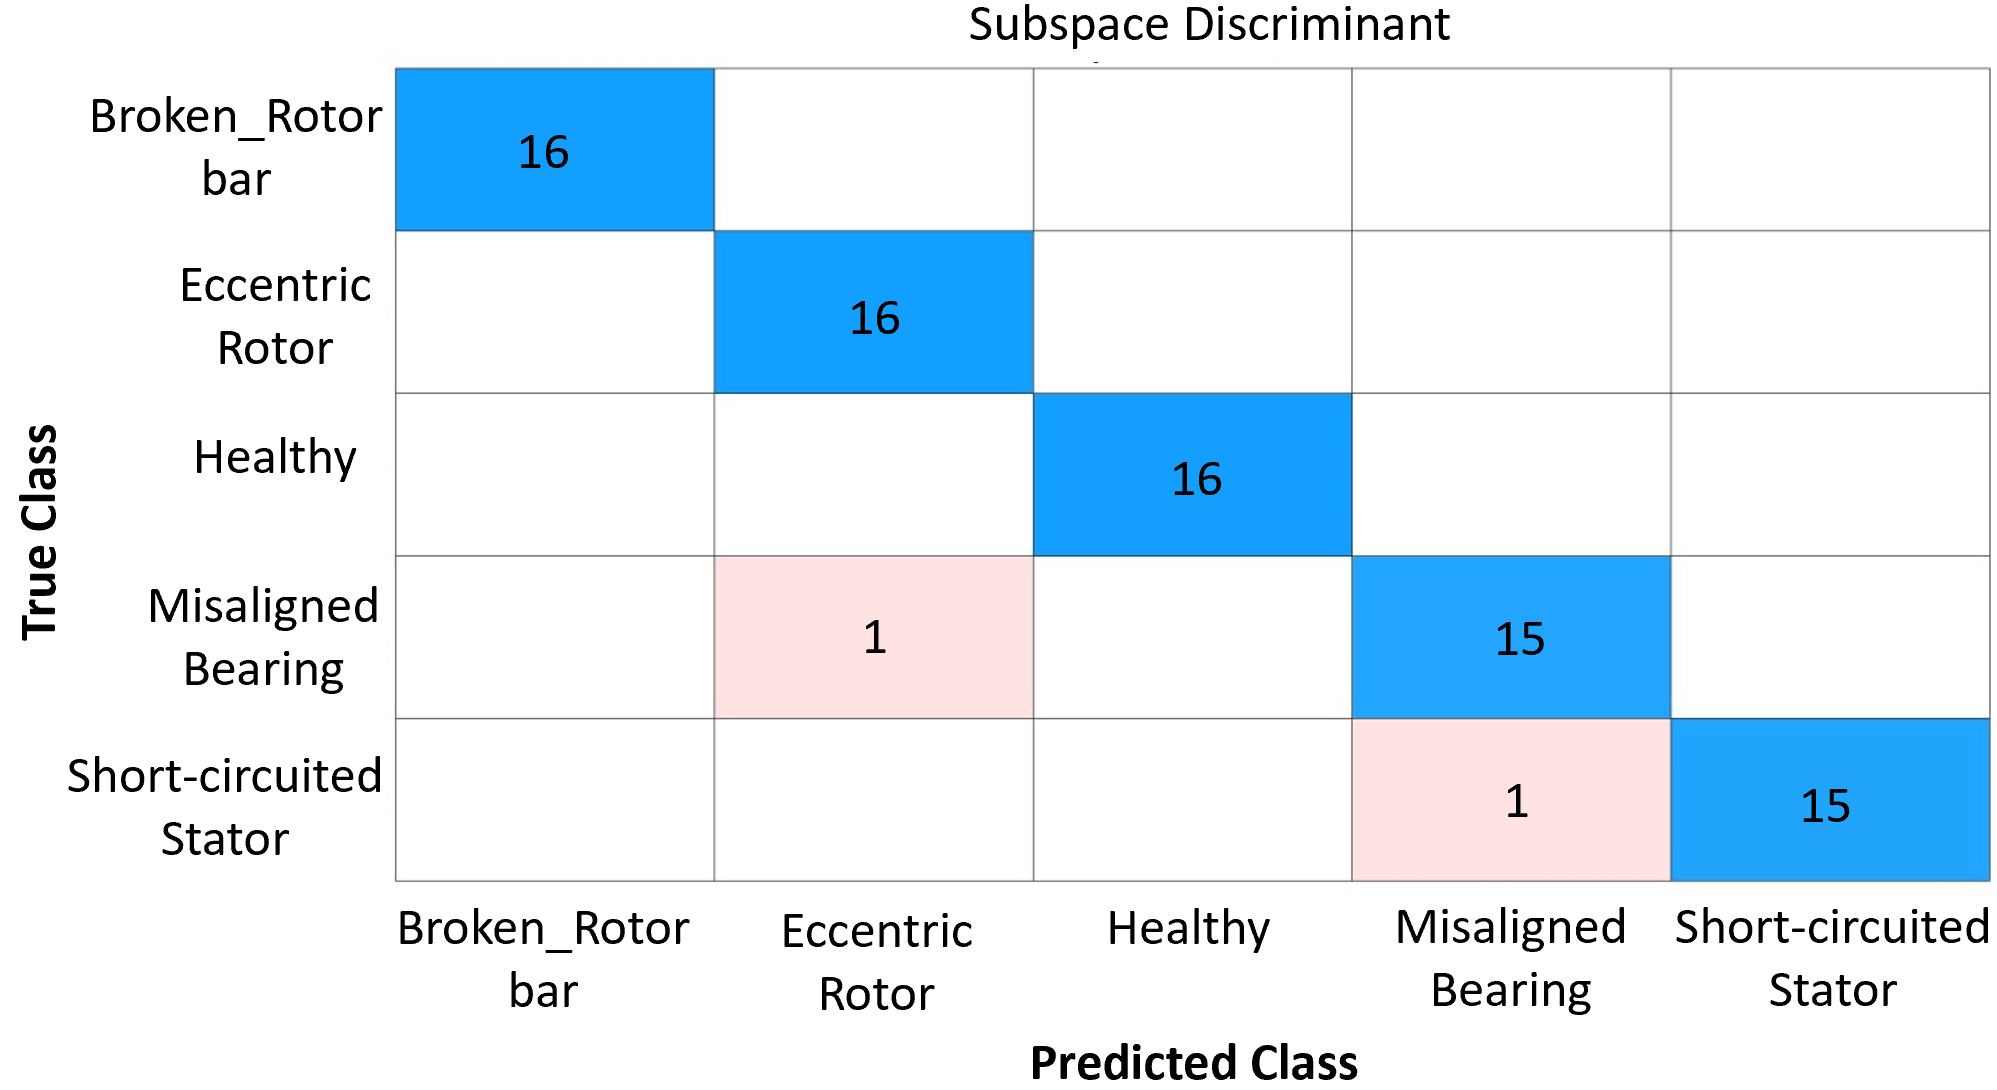
\includegraphics[width=0.47\textwidth]{Figs/attempt11.png}
    \caption{Confusion matrix of fault localization with hybrid DT using Subspace Discriminant method.}
    \label{fig:with_fusion}
\end{figure}


\section{Data Assimilation for Hybrid DT Framework}\label{sec:dataAssimilation}
This section discusses the three key phases for assimilation of real-time and FEM-based datasets, forming the foundation of our hybrid DT framework. \\
\indent\textbf{Phase I - Design Optimization in COMSOL:}
The real-time data for healthy and malfunctioned motors was used to remove discrepancies and calibrate FEM using design optimization and parameter tuning in COMSOL. The design optimization tool adjusts the rotor angular speed of the model $\omega$ in steady state to $\omega_{\text{experimental}}$ of a physical motor. The control variable is the magnetic properties and geometry of the rotor. A nonlinear optimization method, Nelder-Mead~\cite{singer2009nelder}, with optimality tolerance set to $0.01$, is used to minimize our objective function $f(\omega)$:
\begin{equation}
f(\omega) = (\omega_{\text{experimental}} - \omega)^2.
\end{equation}

Three-phase stator current of the experimental dataset serves as reference data for parameter tuning of the FEM. A gradient-based optimization technique named SNOPT (Sparse Nonlinear Optimization) is used for this purpose~\cite{betts1994sparse}. The SNOPT algorithm is used for parameter tuning in COMSOL to calibrate the FEM within a feasibility tolerance of $10^{-4}$. The rotor frequency is tuned to $66.7813$ Hz to match the reference data slip, the stator coil turns are estimated to $2045$, and the stator inductance is estimated to $0.0028$ H.
 


\begin{table}[t!]
\centering
\caption{COMPARISON OF DOF BETWEEN ACTUAL FEM AND THE ROM.}
\label{tab:dof}
\resizebox{0.20\textwidth}{!}{%
\begin{tabular}{c|c}
\textbf{Model} & \textbf{DOF} \\ \hline
\textbf{FEM}   & 105181       \\
\textbf{ROM}   & 2000 
\end{tabular}%
}
\end{table}



\begin{figure}[b!]
    \centering
    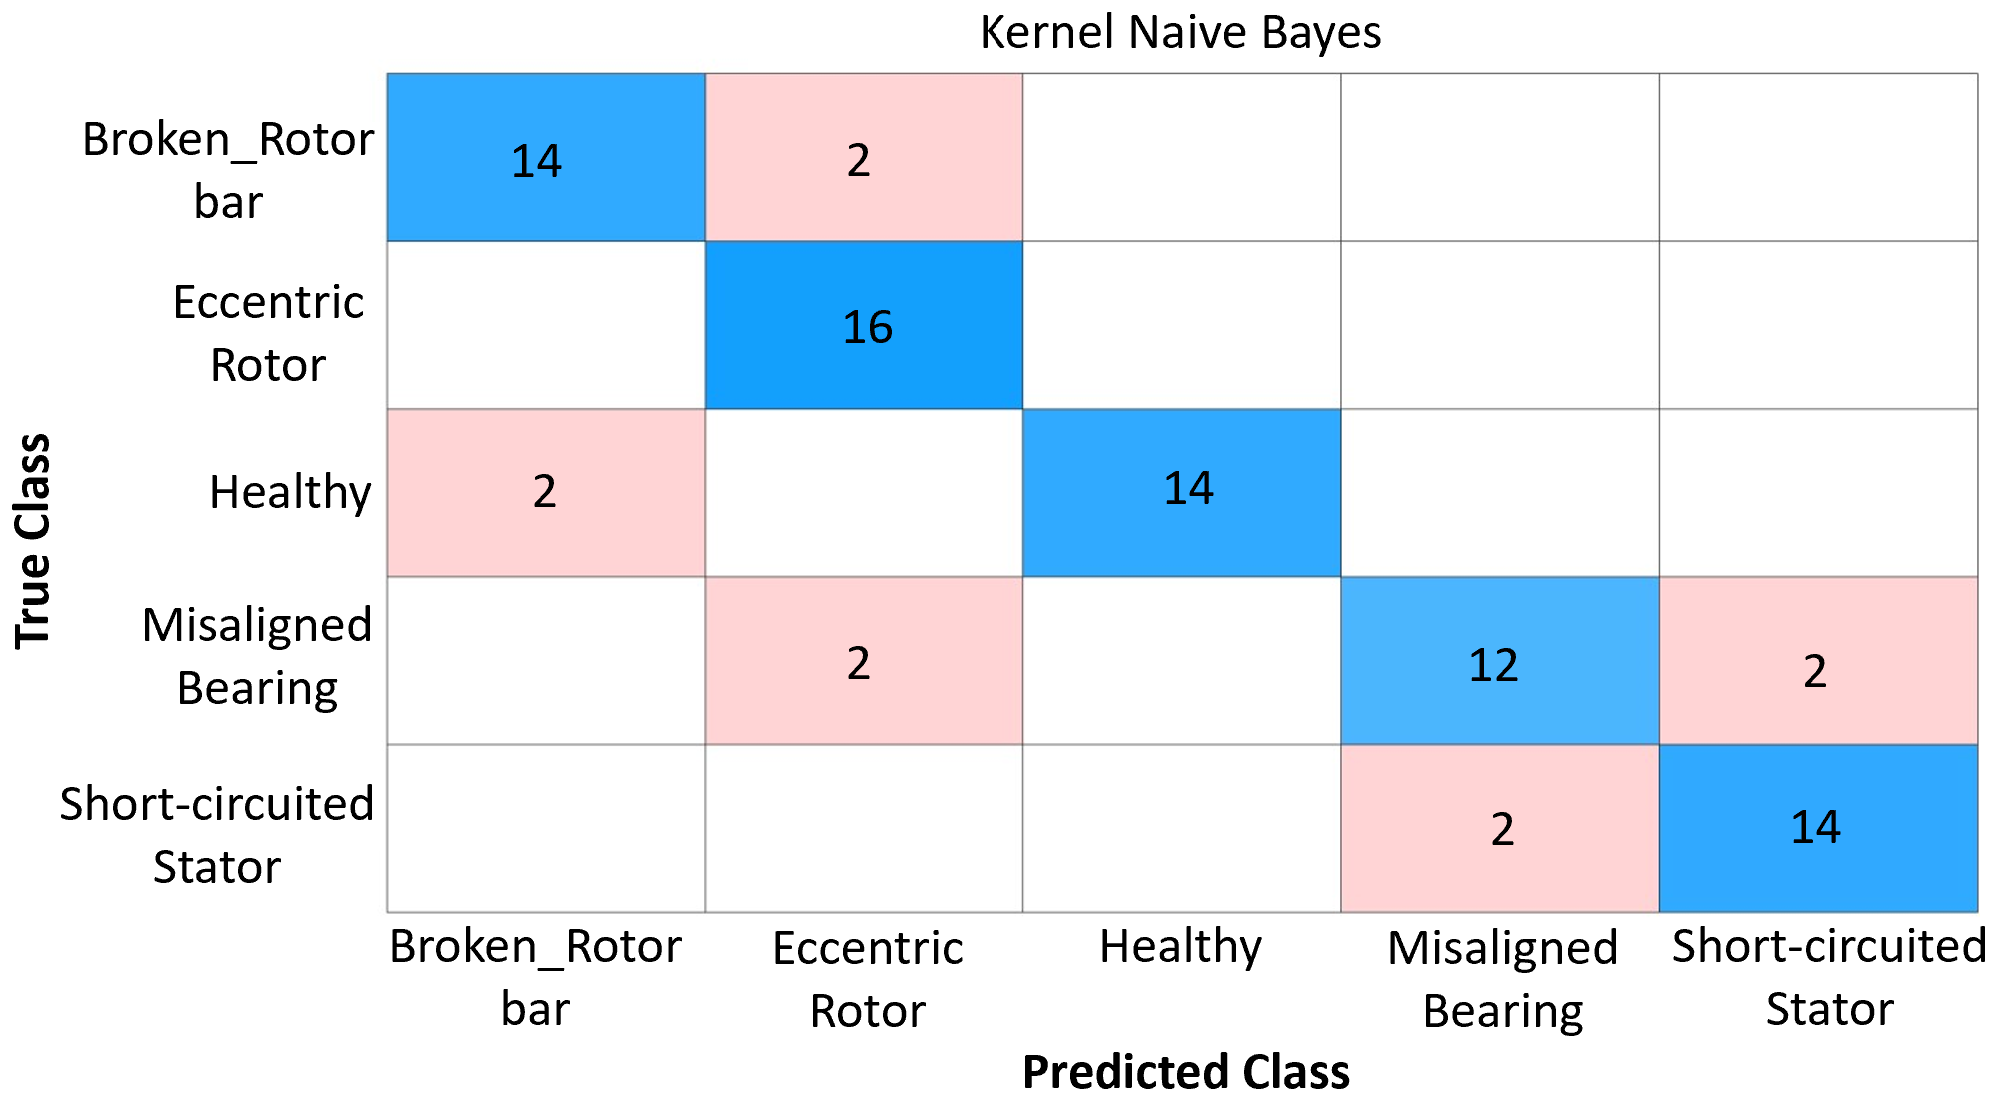
\includegraphics[width=0.45\textwidth]{Figs/attempt12.png}
    \caption{Confusion matrix of fault localization with data-driven DT using Kernel Naive Bayes method.}
    \label{fig:without_fusion}
\end{figure}



\textbf{Phase II - Handling Data Sparsity for Malfunctioned TIM:}
The calibrated FEM generates data sets for sparse variables of physical TIM. The database for short-circuited stator motor is purely synthetic, generated by emulating coil-to-ground faults in the FEM electrical circuit module. The remaining hybrid databases, consisting of real-time and synthetic data points obtained from the COMSOL framework.

\textbf{Phase III - Handling Data Skewness of Experimental and Simulated Testbench:}
The database for torque, angular speed, vibration amplitude, and stator currents with the time-dependent study was generated using a FEM of $40,0000$ data points. Since real-time data sets have $100,000$ data points, SMOTE handles class imbalance for simulated datasets.\\
\indent\textbf{Phase IV - Feature Fusion using CCA for ML Classifiers:} To further enhance the results of our model, we used CCA~\cite{yang2019survey} as another pre-processing step before the input data fed to our ML classifiers. We fused the dataset for synthetic and available real-time data to create a hybrid twin. Data fusion and augmentation plays crucial rule when dealing with multiple inter-correlated outcome variables. This fusion determines features through the orthogonal linear combination of the variables within each dataset to further increase the accuracy of ML models. These models extract the feature sets from cross-covariance matrices and are then trained on those features for fault localization. The objective of CCA is to maximize the correlation coefficient ($\rho$) between two sets of variables, $U$ and $V$ as follows:
\begin{equation}
\quad \rho = \text{corr}(U, V).
\label{eq: 1}
\end{equation}

The following constraints ensure that the covariance between $U$ and $V$ equals $0$, indicating their orthogonality, and that their variance equals $1$, indicating they are normalized, as follows:
\begin{equation}
\text{Cov}(U, V) = 0,
\label{eq: 4}
\end{equation}
\begin{equation}
\quad \text{Var}(U) = 1 \text{ , } \text{Var}(V) = 1.
\label{eq: 2}
\end{equation}


We fused the dataset for synthetic and available real-time data to create a hybrid DT. Data fusion and augmentation is helpful for multiple inter-correlated outcome variables. This fusion determines features through the orthogonal linear combination of the variables within each dataset to further increase the accuracy of our ML models.
\begin{figure}[t!]
    \centering
    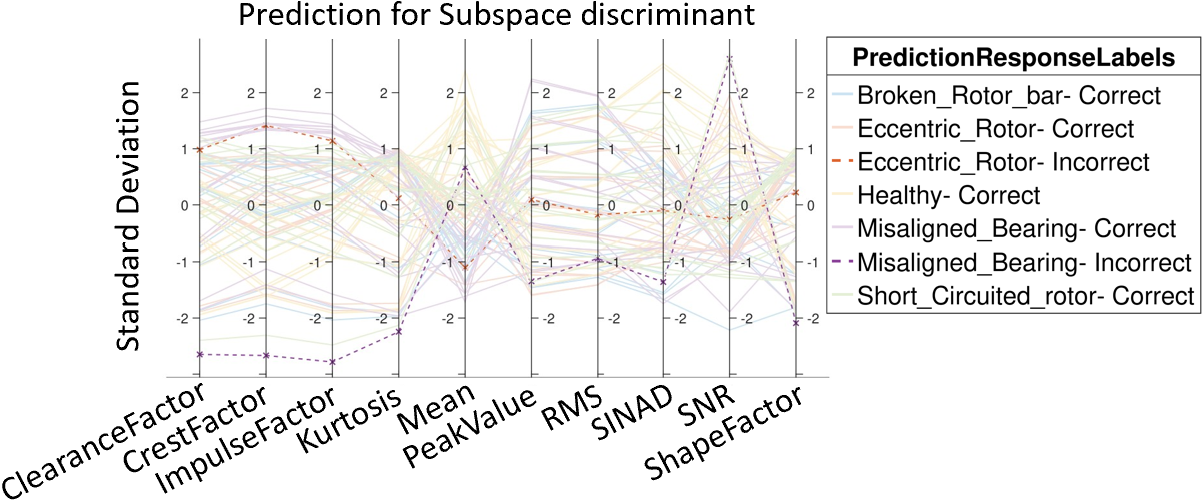
\includegraphics[width=0.45\textwidth]{Figs/JAZZ15.png}
    \caption{Prediction response for subspace discriminant curve showing correct and incorrect labels during each training epoch.}
    \label{fig:fusion_prediction}
\end{figure}
\section{Hybrid DT for Fault Localization} \label{sec:FaulLocalization}
We first performed feature extraction for ML classifiers for fault localization. Non-linear feature extraction and rotating machinery features were extracted from both datasets (fused and without fusion). Moreover, we applied the Autoregressive model for modeling time-series data of stator currents and voltages. Welch's method~\cite{welch1967use} is applied to estimate the power spectral density and analyze frequency domain characteristics of torque and vibration signals. After extracting features, we performed feature ranking based on one-way ANOVA~\cite{st1989analysis}. It is a statistical tool used to compute the variance of features and rank the features according to their potential usefulness for fault localization. Moreover, we estimated bearing fault features and geometric lattice dataset for improved fault prediction and fault analysis in the motor.
Then, these spectrum features were plotted against classification learners. Table~\ref{tab: accuracies} displays the performance accuracy corresponding to the various ML models. All the ML models were trained simultaneously using parallel pool threads. 

\begin{table}[b!]
\centering
\caption{COMPARISON OF ACCURACY(ACC) FOR FAULT LOCALIZATION USING ML CLASSIFIERS.}
\label{tab: accuracies}
\resizebox{\columnwidth}{!}{%
\begin{tabular}{ccc}
\hline
\textbf{ML Classifiers} & \textbf{Hybrid Model }& \textbf{Data-Driven Model } \\ 
&  ACC ($\%$) & ACC ($\%$)\\ \hline
\textbf{K-Nearest Neighbors (Coarse)}         & 83.28          & 81.71          \\
\textbf{K-Nearest Neighbors (Cubic)}         & 84.17          & 80.17          \\
\textbf{Fine Tree} \cite{wu2014ml}                           & 80.97          & 77.14          \\
\textbf{Optimizeable Support Vector Machines} \cite{hearst1998support} & 85.10          & 80.82          \\
\textbf{Kernel Naive Bayes}                  & 87.23          & \textbf{87.5} \\
\textbf{Subspace Discriminant}  \cite{zhang2007discriminant}              & \textbf{97.5} & 84.67          \\ \hline
\end{tabular}%
}
\end{table}








\section{Hybrid DT for Offset Prediction by Load Variation}\label{sec:OffsetPrediciton} 
Besides common electrical and mechanical faults, an imbalance in the motor's applied load due to fluctuating load conditions is also a major risk for TIM’s normal operation. The differences between the rotor's centers of gravity (COG) and the connected load cause forces to act along their rotational axes. The centrifugal force resulting from the load unbalance is proportional to the load mass. The motor is tested under six loading conditions ranging from $6$ to $35$ grams to determine the unbalanced fault. Accelerometers planted in the radial, axial, and tangential directions are employed for vibrational analysis to determine load imbalance. Table~\ref{tab: accuracies_deep} shows the accuracies of various Deep Learning (DL) and ML models trained for offset prediction. Deep neural networks (DNN) outperformed the ML model, obtaining ninety-nine percent accuracy. It is observed that the feature extraction for ML models becomes tedious, and the accuracy falls for the massive dataset.

\begin{figure}[t!]
    \centering
    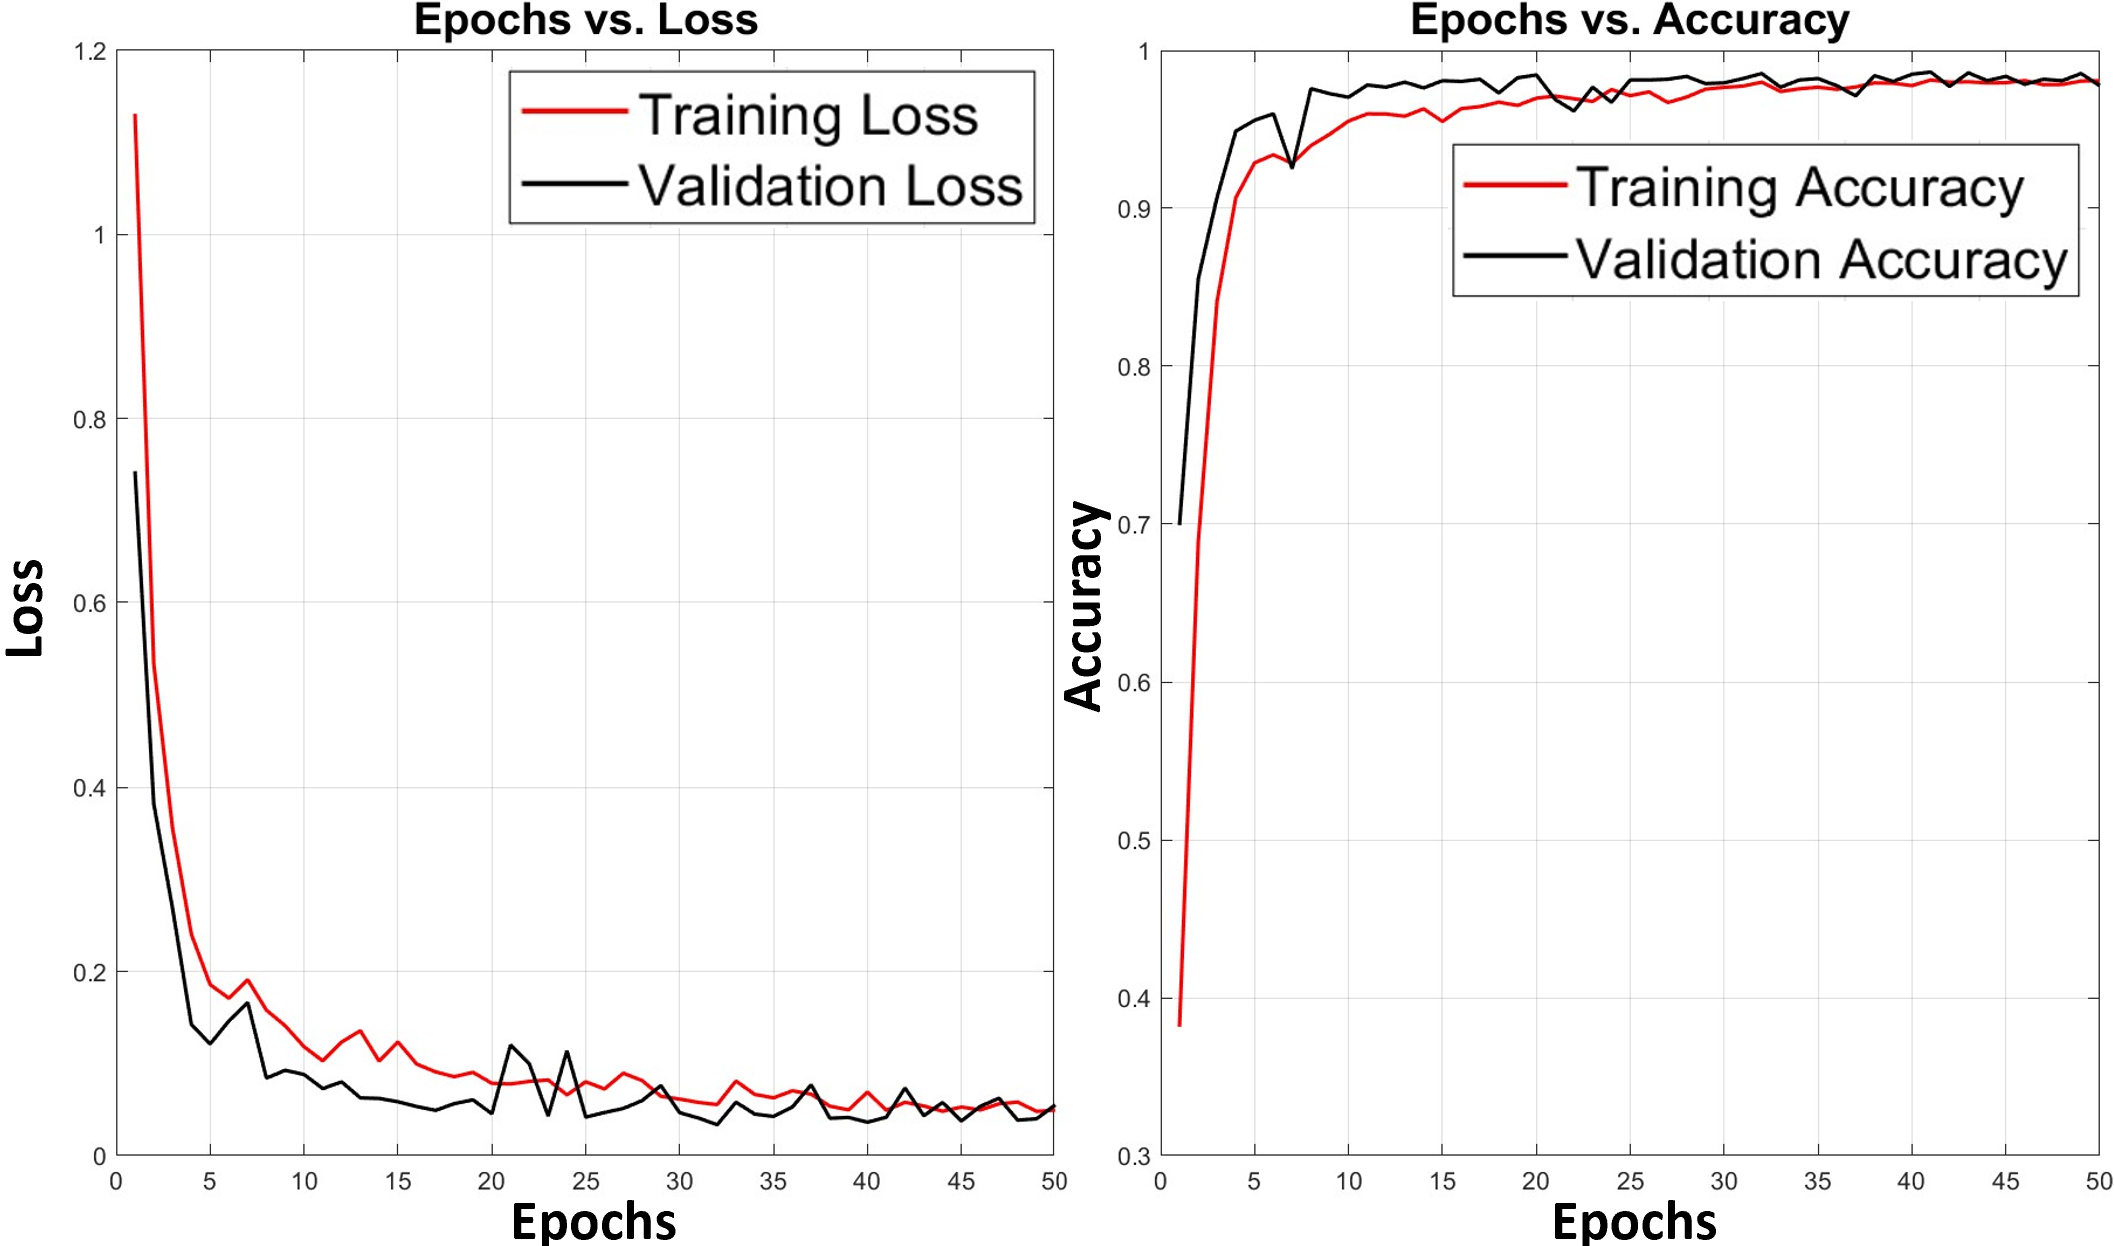
\includegraphics[width=0.45\textwidth]{Figs/Jazz4.png}
    \caption{Convergence of loss and accuracy curves for offset prediction using DL model over 50 training epochs.}
    \label{fig:Deep_Learning}
\end{figure}


\begin{table}[b!]
\centering
\caption{ACCURACY COMPARISON FOR OFFSET PREDICTION USING ML AND DL MODELS.}
\resizebox{\columnwidth}{!}{%
\begin{tabular}{ccc}
\hline
\textbf{ML and DL Models} & \textbf{Hybrid Model } & \textbf{Data-Driven Model } \\ 
& ACC ($\%$) & ACC ($\%$)\\ \hline
\textbf{K-Nearest Neighbors (Coarse)} \cite{guo2003knn}       & 88.71          & 84.67          \\
\textbf{Recurrent Neural Networks}  \cite{schafer2007recurrent}       & 89.10          & 85.39          \\
\textbf{Random Forest}              \cite{biau2012analysis}              & 80.97          & 77.14          \\
\textbf{Support Vector Machines} \cite{hearst1998support} & 85.18          & 83.29          \\
\textbf{Kernel Naive Bayes}  \cite{tuytelaars2011nbnn}                & 87.69          & 85.47 \\
\textbf{DL Model (CNN)}  \cite{miikkulainen2019evolving}              & \textbf{98.87} & \textbf{96.38}          \\ \hline
\end{tabular}%
}
\label{tab: accuracies_deep}
\end{table}


\



\section{Quantitative Analysis}\label{sec:quantitativeAnalysis}

Table \ref{tab: accuracies} compares the accuracies of ML classifiers between hybrid DT and data-driven DT. The models for hybrid DT demonstrated greater accuracies compared to data-driven DT. The best model for hybrid DT was Subspace Discriminant, with an accuracy of 97.5\%. The data-driven model showed less accurate results as expected by our experimentation, with the best model being Kernel Naive Bayes, showing an accuracy of 84.18\%. The confusion matrix of hybrid DT for the best model (Subspace Discriminant) is shown in Fig.~\ref{fig:with_fusion}. The confusion matrix of the hybrid DT for the best model (Kernel Naive Bayes) is shown in Fig.~\ref{fig:without_fusion}. The prediction response of Subspace Discriminant is demonstrated in Fig.~\ref{fig:fusion_prediction}, where the two dashed plots represent incorrect predictions for misaligned bearing and eccentric rotor.

We initially deployed ML classifiers for offset detection, and K-Nearest Neighbors (Course) achieved the highest accuracy of 88.71\% among the ML classifiers, as listed in Table~\ref{tab: accuracies_deep}. Due to the scalability of large datasets, a convolutional neural netowrk (CNN) was deployed to overcome the feature extraction problem. CNN achieved the highest accuracy score of 98.87\%. Despite the computational trade-off between the ML and DL algorithms, we observed that the DL algorithms outperformed the ML classifiers in hybrid and data-driven modeling. Fig.~\ref{fig:Deep_Learning} demonstrates the accuracy and loss curves of our DT. Training and validation data converge over the course of $50$ training epochs. 

\section{Conclusion and Future Work}\label{sec:conclusion}
This paper proposes a hybrid DT for fault localization in TIM. FEMs are calibrated to the physical system using non-linear design optimization methods like SNOPT and Nelder–Mead. The state-of-the-art model reduction algorithm of the sssMOR toolbox is used to reduce the computational resources of FEM by generating an adequate mathematical subspace within 0.4464\% accuracy. SMOTE harmonizes data distribution, while CCA is used for feature fusion. Autoregressive and Welch’s models are used for feature extraction, and various ML, optimization ensemble, and DL models are trained for fault localization. DL model has the highest accuracy, 98.87\% for offset prediction in TIM. 

Future works involve incremental ML and parallel computing approaches, enabling dynamic updates of DT as new data becomes available. 
Further advancements can be made by exploring other methodologies to bridge the gap between physics-driven and data-driven modeling. Data fusion techniques can also be used to model combinations of multiple faults within a particular TIM. 

\bibliographystyle{IEEEtran}
\bibliography{ref}
	
\end{document}
